A very high-level overview of the topic is given here.

\lipsum[1]

\section{circRNAs}
This section describes what circRNAs are, how they are formed, and what their
functions are. It also gives insights into the current state of research.

\subsection{Biogenesis}
During standard gene expression, pre-mRNA is transcribed from DNA. Splicing then
removes introns and joins exons to produce mature mRNA
\supercite{black_mechanisms_2003}. In conventional splicing, an upstream 5'
splice site (donor) connects to a downstream 3' splice site (acceptor), forming
linear mRNA (\cref{fig:circRNA_splicing}a). Conversely, for circRNAs, a
downstream 5' splice site connects to an upstream 3' splice site in reverse
order across at least one exon \supercite{chen_expanding_2020}. This
backsplicing process is - just like conventional splicing - catalyzed by the
canonical spliceosome \supercite{starke_exon_2015} and results in a circular RNA
molecule (\cref{fig:circRNA_splicing}b).

\subsubsection{Models}
Two models have been proposed to explain the formation of circRNAs: The direct
backsplicing model and the lariat-intermediate model.
% TODO: Add more details, reference {fig:circRNA_splicing}d

\subsubsection{Alternative splicing}
In conventional splicing, introns are removed and exons are joined linearly.
However, in some cases, exons are skipped or introns are retained, leading to
alternative mature mRNA transcripts based on the same pre-mRNA. This process is
known as alternative splicing \supercite{nilsen_expansion_2010}. Similarly,
circRNAs can be subject to alternative splicing. This can result in the
structures shown in \cref{fig:circRNA_splicing}e and
\cref{fig:circRNA_splicing}f.

\begin{figure}[ht]
    \centering
    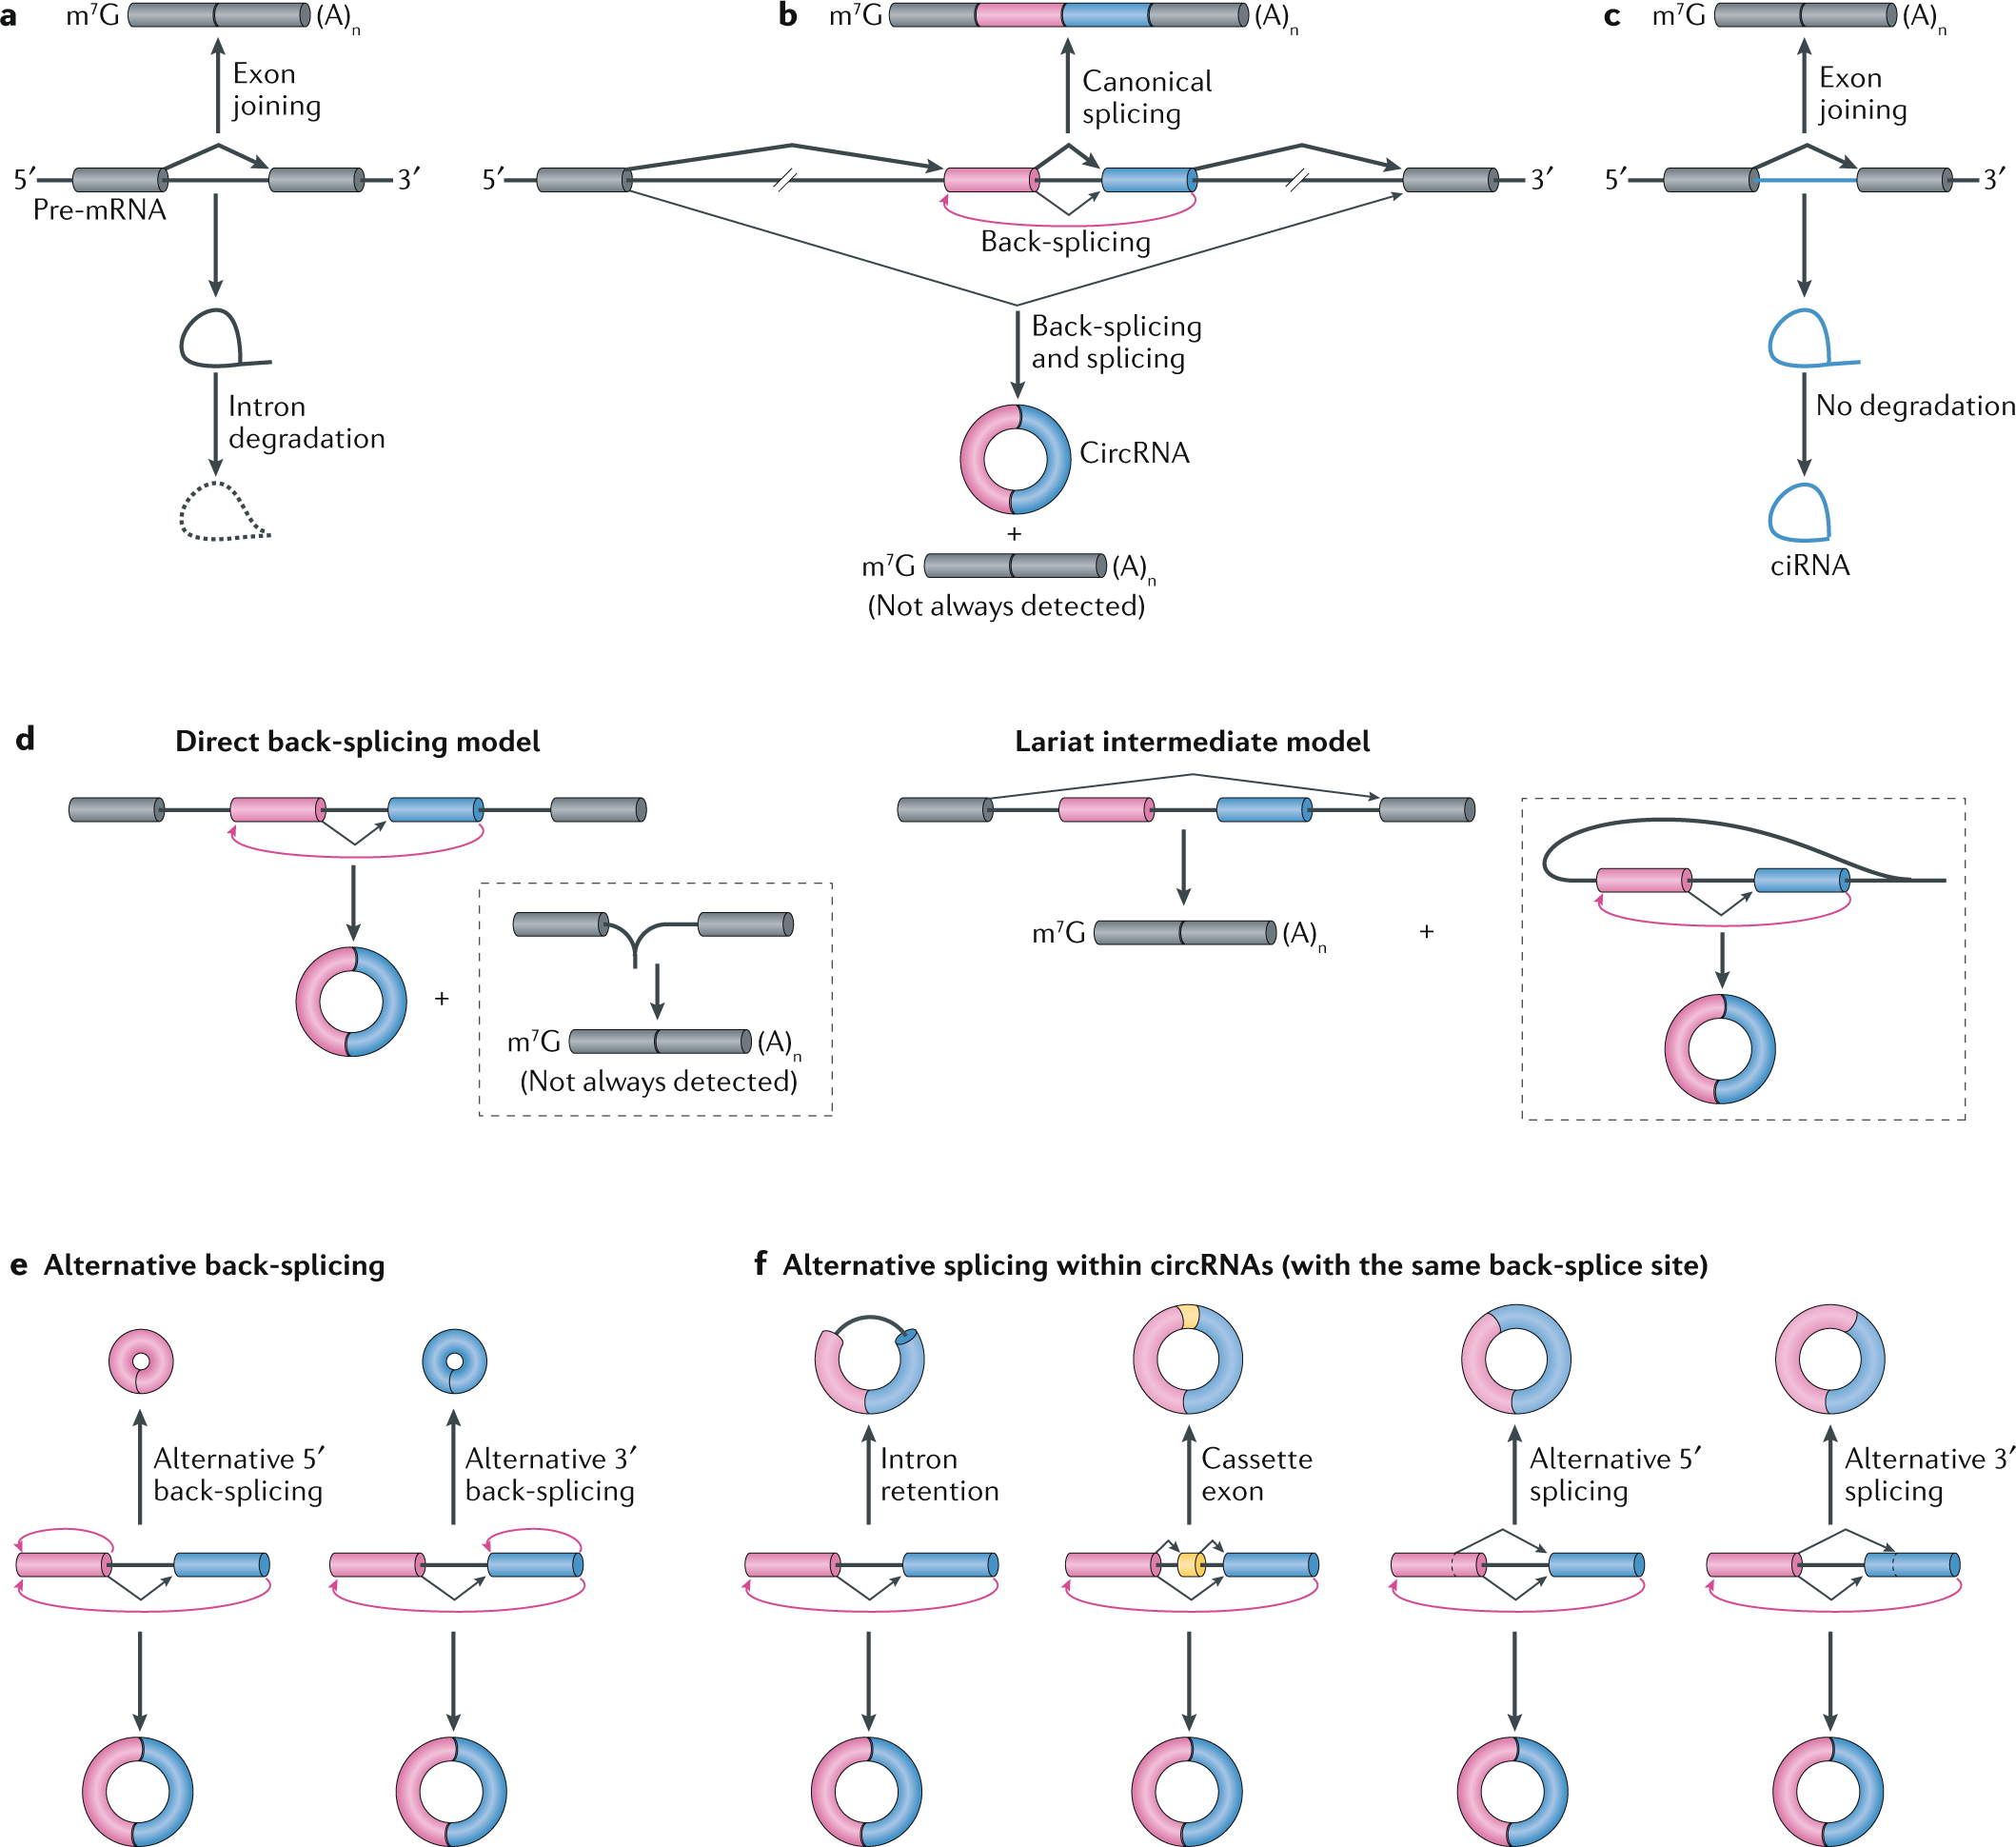
\includegraphics[width=\textwidth]{chapters/background/figures/circRNA-splicing.png}
    \caption{Splicing of circRNAs} % TODO: Add detailed caption
    \label{fig:circRNA_splicing}
\end{figure}

\subsection{circRNA types}
\subsubsection{Circular intronic RNAs (ciRNAs)}
Introns typically form a lariat shape during conventional splicing, which is
generally debranched and degraded soon after splicing
(\cref{fig:circRNA_splicing}a). However, in some cases, introns evade
debranching and instead form covalently bonded circular RNA molecules
(\cref{fig:circRNA_splicing}c), known as circular intronic RNAs (ciRNAs)
\supercite{chen_expanding_2020,zhang_circular_2013}.

\subsubsection{Exonic circular RNAs (EcircRNAs)}
EcircRNAs are generated from exon-skipping events. Here, the lariat contains at
least one exon and potentially multiple introns. The introns are subsequently
removed through internal splicing, producing a circular RNA molecule composed
solely of exonic sequences \supercite{xiao_circular_2022, li_biogenesis_2018}.

\subsubsection{Exon-intron circular RNAs (EIcircRNAs)}
The formation of EIcircRNAs is similar to that of EcircRNAs, with the exception
that introns are not completely removed during splicing, resulting in a circular
RNA molecule containing both exonic and intronic sequences
\supercite{xiao_circular_2022}.

\subsection{Biological functions}
circRNAs have emerged as key players in various biological processes, showcasing
a wide range of functions that contribute substantially to cellular regulation.

\subsubsection{Micro RNA sponging}
MicroRNAs (miRNAs) are small non-coding RNAs that regulate gene expression
\supercite{bartel_micrornas_2009}. They can bind to target mRNAs and either
inhibit translation or promote degradation \supercite{bartel_micrornas_2009}.
Competing endogenous RNAs (ceRNAs) can bind to miRNAs, preventing them from
binding to their target mRNAs \supercite{tay_multilayered_2014}. circRNAs can
function as ceRNAs by sponging miRNAs, thereby regulating gene expression
\supercite{xiao_circular_2022}.

\subsubsection{Protein interactions}
This subsubsection describes how circRNAs can bind to proteins.

\subsubsection{Translation into peptides}
In the canonical initiation of translation, ribosomes bind to the 5' cap of an
mRNA \supercite{hinnebusch_mechanism_2012}. Because circRNAs are circular and
lack a 5' cap, they were long thought to be non-coding
\supercite{bao_regulatory_2019,greene_circular_2017}. However, research has
shown that circRNAs with internal ribosome entry sites can indeed be translated
into proteins \supercite{chen_expanding_2020}:

\paragraph{Internal ribosome entry sites (IRES)}
In 1988, researchers discovered that certain viral and cellular mRNAs contain
sequences allowing ribosomes to initiate translation without a 5' cap
\supercite{pelletier_internal_1988, jang_segment_1988}. These sequences are
known as internal ribosome entry sites (IRES). In 1995, Chen and Sarnow
demonstrated that artificially engineered circRNAs containing an IRES sequence
are translated into peptides \supercite{chen_initiation_1995}. Later, it
was found that some circRNAs naturally possess IRES sequences and can thus be
translated into peptides
\supercite{chen_expanding_2020,legnini_circ-znf609_2017,pamudurti_translation_2017}.
A concrete example for an IRES is the consensus motif for
N\textsuperscript{6}-methyladenosine modification \supercite{yang_extensive_2017}.

\paragraph{N\textsuperscript{6}-methyladenosine (m\textsuperscript{6}A)}
% General introduction to m6A
m\textsuperscript{6}A is the most abundant base modification in eukaryotic RNA
\supercite{yang_extensive_2017,li_pivotal_2014,wei_methylated_1975}. Research
has shown that m\textsuperscript{6}A modification can affect localization,
splicing, translation and degradation of RNA molecules
\supercite{yue_rna_2015,meyer_dynamic_2014}. The effect of m\textsuperscript{6}A
modification on translation is particularly interesting, as it has been shown
that m\textsuperscript{6}A modifications in 3' UTRs can enhance translation
efficiency\supercite{wang_n6-methyladenosine_2015}, while m\textsuperscript{6}A
modifications in 5' UTRs can promote cap-independent translation, especially in
heat shock stress\supercite{zhou_dynamic_2015,meyer_5_2015}.

% Build bridge to IRES-dependent mechanism
m\textsuperscript{6}A modifications mostly occur in the consensus motif
RRm\textsuperscript{6}ACH (R = purine, H = non-guanine base)
\supercite{csepany_sequence_1990,harper_sequence_1990}, which has been found to
be enriched in circRNAs \supercite{yang_extensive_2017}. In circRNAs, a single
m\textsuperscript{6}A modification is often enough to initiate translation
\supercite{yang_extensive_2017}.

\subsubsection{Gene regulation}
As we have seen, circRNAs can interact with miRNAs and proteins.

\subsection{Potential applications}
This subsection describes potential applications of circRNAs.

\subsubsection{Biomarkers}
Since circRNAs do not possess 5' caps or 3' polyA tails, they are not prone to
RNase R digestion. Thus, they are generally more stable and have longer
half-lives than linear RNAs \supercite{kristensen_biogenesis_2019}.

\subsection{Existing research}
This subsection describes the current state of research on circRNAs.

\section{totalRNA sequencing}
This subsection describes the sequencing method used to identify circRNAs.

\lipsum[2]

\section{Breast cancer}
This section describes what breast cancer is, how it is diagnosed, and what the
current treatment options are. It also gives insights into the current state of
research.

\subsection{Abundance}
Breast cancer is the most common cancer

\subsection{Causes}

\section{Estrogen signaling}
This section describes what estrogen is, how it affects breast cancer, and what
the current treatment options are. It also gives insights into the current state
of research.

\lipsum[4]

\section{Related work}
This section describes related work on circRNAs, breast cancer, and estrogen
signaling.

\subsection{circRNA-sponging pipeline}
This subsection describes a pipeline for identifying circRNA sponges.